\section{Remote monitoring: troubleshooting}
\label{scenario:rm-troubleshooting}

\npar The ``Bill payment is received'' scenario mainly describes telephone
support after something went wrong with a remote module. Because this is not
software, we show what will happen when a measurement goes missing. Figure
\ref{fig:scenario-5-3-3} shows a sequence diagram for this scenario.

\begin{figure}[H]
	\begin{centering}
		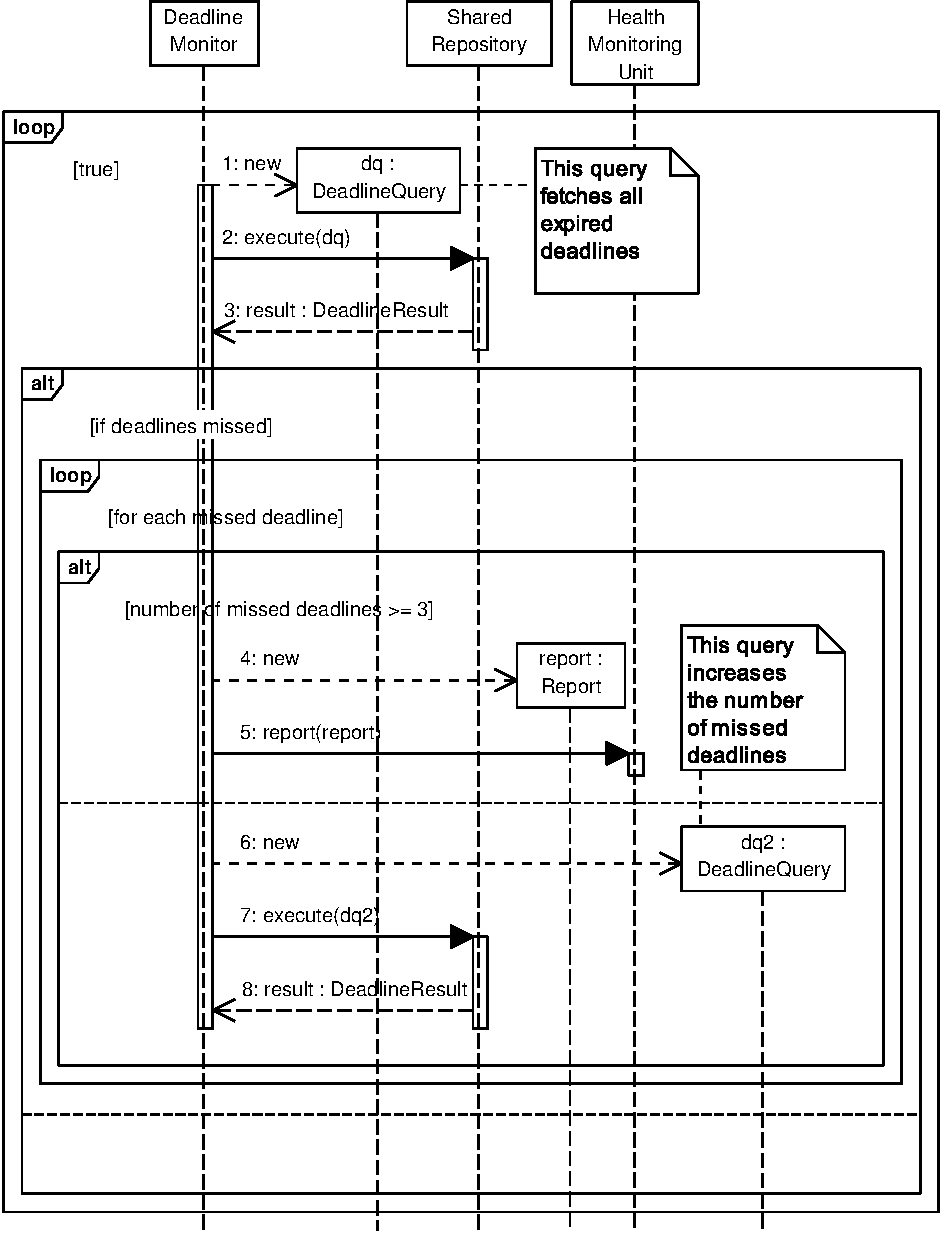
\includegraphics[width=\textwidth]{figs/scenario-5-3-3.pdf}
		\caption{Sequence diagram of the ``Remote monitoring: troubleshooting"
		Scenario}
		\label{fig:scenario-5-3-3}
	\end{centering}
\end{figure}

\npar At the arrival of a measurement trame, the deadline for the next trame is
calculated (update interarrival time + 10 minutes). Periodically, the
missed deadline are fetched from the database. For every device that missed the
deadline, a counter is increased. Whenever a counter for a device reaches 3, a
ReMeS operator is notified through the Health Monitoring Unit. 

\npar If, however, a trame arrives after the deadline, the counter is reset and
the next deadline is calculated and stored.
